\documentclass{article}
\usepackage[chinese, draft]{complex2}
\usepackage{enumitem}
%\usepackage[chinese, draft]{../Complex2}
\setlength{\headheight}{12.13004pt}
\def\ntitle{2021 年校际数学比赛参考解答}
\def\ndescription{此卷有 10 道题目:
题 1 -- 3 每题 8 分;
题 4 -- 6 每题 10 分;
题 7 -- 10 每题 12 分.
请务必留意文末的声明.}
\def\ndate{August, 2021}
%\def\nauthor{Complex2- Liu}
\def\nemail{complex2liu@stu.pku.edu.cn}
\def\nmotto{There is more than one way to skin a cat.}
\allowdisplaybreaks
\begin{document}
\input{~/tex/titlepage.tex}

\begin{prob}
简化以下的和 $1 + \sum_{n=1}^{2021}(-1)^n \frac{n^2 + n + 1}{n!}$.
\end{prob}

\begin{soln}
想办法裂项:
\begin{equation}
\label{eq1}
a_n \defeq \frac{n^2 + n + 1}{n!} = \frac{n(n-1) + 2n + 1}{n!} = \frac{1}{(n-2)!} + \frac{2}{(n-1)!} + \frac{1}{n!}.
\end{equation}
注意到连续的三项会把分母为 $n!$ 的那一项给消掉, 所以
\begin{align*}
1 + \sum_{n=1}^{2021}(-1)^na_n &= 1 - a_1 + a_2 + (-a_3 + a_4 - \cdots)\\
&=1 - a_1 + a_2 + \left(\frac{(-1)^3}{(3-2)!} + \frac{(-1)^3\cdot 2}{(3-1)!} + \frac{(-1)^4}{(4-2)!} +\right.\\
&\phantom{=========}\left.\frac{(-1)^{2020}}{2020!} + \frac{(-1)^{2021}\cdot 2}{(2021-1)!} + \frac{(-1)^{2021}}{2021!}\right)\\
&= 1 - 3 + \frac{7}{2} - 1 - \frac{1}{2} - \frac{1}{2020!} - \frac{1}{2021!}\\
&= \boxed{-\frac{2022}{2021!}.}
\end{align*}
\end{soln}

\begin{rem}
考基本的代数变形.
\end{rem}

\begin{prob}
记 $P(x) = x^2 + ax + b$, 其中 $a,b \in [-2,2]$.
当 $a,b$ 在闭区间 $[-2,2]$ 上变动时,
求二次方程 $P(x) = 0$ 的实数解的取值范围.
\end{prob}

\begin{soln}
$\Delta = a^2 - 4b \le 12$. 易知答案为
\[\boxed{\frac{-2 - \sqrt{12}}{2}} \le \frac{-a \pm \sqrt{\Delta}}{2} \le \boxed{\frac{2 + \sqrt{12}}{2}.}\]
\end{soln}

\begin{prob}
在 $xy$ 平面上, 记 $f(a,b)$ 为点 $(a,b)$ 到直线 $\ell: 3x + 4y = 1$ 的距离.
当 $a,b$ 走遍所有整数且 $(a,b)$ 不在直线 $\ell$, 确定 $f(a,b)$ 的最小值.
\end{prob}

\begin{soln}
回忆点到直线的距离公式
\begin{equation}
\label{eq2}
d = \abs*{\frac{3a + 4b - 1}{\sqrt{3^2 + 4^2}}}.
\end{equation}
题目的要求为 $a,b \in \ZZ$ 且 $3a + 4b - 1 \ne 0$,
注意到 $3a + 4b - 1 \in \ZZ$, 所以
\[d_{\mathrm{min}} = \boxed{\frac{1}{5}.}\]
\end{soln}

\begin{prob}
将边长为 $n$ 的等边三角形的每条边等分 $n$ 份,
然后用平行这三边的线段连起这些等分点,
得出一些由边长为 $1$ 的等边三角形所组成的图形 $S_n$.
设图形 $S_n$ 共有 $N_n$ 个边长 $1$ 至 $n$ 的等边三角形.
下图给出当 $n=1,2,3$ 的图形, $N_1 = 1, N_2 = 5$.
试找出用 $n$ 表示 $N_n$ 的公式.
\begin{center}
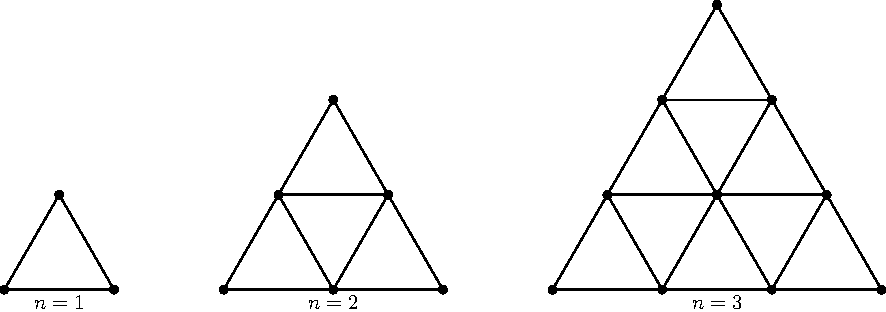
\includegraphics[scale=0.5]{p4.pdf}
\end{center}
\end{prob}

\begin{soln}
我们把等边三角形划分为两类: 一类头朝上, 一类头朝下,
以 $n=2$ 为例, 有 $4$ 个头朝上的三角形, $1$ 个头朝下的三角形.
设 $a_i(n)$ 为 $S_n$ 中边长为 $i$ 的头朝上的等边三角形的个数.
注意到一个等边三角形被它的一条水平方向的边, 以及头的朝向给唯一决定, 所以
\begin{equation}
\label{eq3}
a_i(n) = (n-i+1) + (n-1-i+1) + \cdots + 1.
\end{equation}
以 $n=3$ 为例, 最底层(记为第 $0$ 层)长度为 $3$,
贡献 $3-i+1$ 个边长为 $i$ 的头朝上的等边三角形,
上一层(记为第 $1$ 层)长度为 $2$,
贡献 $2-i+1$ 个边长为 $i$ 的头朝上的等边三角形.
我们有
\begin{align*}
&a_1(n)=1 + 2 + \cdots + (n-1) + n\\
&a_2(n)=1 + 2 + \cdots + (n-1)\\
&\cdots\\
&a_n(n)=1.
\end{align*}
换序求和便知
\begin{align*}
\sum_{i=1}^n a_i(n) &= \sum_{i=1}^n i\cdot(n+1-i) = (n+1)\cdot\sum_{i=1}^n i - \sum_{i=1}^n i^2\\
&=(n+1)\cdot \frac{n(n+1)}{2} - \frac{n(n+1)(2n+1)}{6}\\
&=\frac{n(n+1)(n+2)}{6}.
\end{align*}

设 $b_i(n)$ 为 $S_n$ 中边长为 $i$ 的头朝下的等边三角形的个数.
对于第 $j$ 层, 它的长度为 $n-j$,
它不可能贡献边长 $> j$ 的头朝下的等边三角形.
类似于 \cref{eq3} 我们可以得到
\begin{equation}
\label{eq4}
b_i(n) = (n-i-i+1) + \cdots + 1,
\end{equation}
其中 $n-i-i+1$ 由第 $i$ 层贡献. 我们有
\begin{align*}
b_1(n) &= 1 + 2 + \cdots + (n-3) + (n-2) + (n-1)\\
b_2(n) &= 1 + 2 + \cdots + (n-3)\\
&\cdots\\
b_i(n) &= 1 + 2 + \cdots + (n-2i+1).
\end{align*}
不难计算得
\begin{equation}
\label{eq5}
\sum_i b_i(n) = \begin{cases}
\frac{(n+1)(n-1)(2n+3)}{24}, \quad &\text{if $n$ is odd};\\
\frac{n(n+2)(2n-1)}{24}, \quad &\text{if $n$ is even}.
\end{cases}
\end{equation}
这里以 $n = 2k-1$ 为例, 此时
\begin{align*}
b_1(n) &= 1 + 2 + \cdots + (n-3) + (n-2) + (n-1),\\
&\cdots\\
b_{k-2}(n) &= 1 + 2 + 3 + 4 + 5 + 6,\\
b_{k-1}(n) &= 1 + 2 + 3 + 4,\\
b_{k}(n) &= 1 + 2.
\end{align*}
所以
\[\sum_i b_i(n) = \sum_{i=1}^{k-1}(k-i)(-1+4i)=\frac{k(k-1)(4k+1)}{6}.\]
We finally conclude that
\[\boxed{N_n = \begin{cases}
\frac{(n+1)(2n^3 + 3n - 1)}{8}, \quad &\text{if $n$ is odd};\\
\frac{n(n+2)(2n+1)}{8}, \quad &\text{if $n$ is even}.
\end{cases}}\]
\end{soln}

\begin{prob}
\begin{enumerate}[label=(\roman*)]
\ii 设 $x,y,z$ 为正数, 求证 $x^{x-y}y^{y-z}z^{z-x} \ge 1$.
\ii 设 $a,b,c$ 为正数, 求证 $a^4 + b^4 + c^4 \ge a^2bc + ab^2c + abc^2$.
\end{enumerate}
\end{prob}

\begin{soln}
(i) 不妨设 $x=\min\{x,y,z\}, y=x+a, z=x+b$, 其中 $a,b \ge 0$.
问题归结为
\begin{equation}
\label{eq6}
1 \le x^{-a}(x+a)^{a-b}(x+b)^b = \left(\frac{x+a}{x}\right)^a\left(\frac{x+b}{x+a}\right)^b = \left(\frac{x+a}{x}\right)^{a-b}\left(\frac{x+b}{x}\right)^b.
\end{equation}
容易看出, 无论 $a \ge b$ 还是 $a \le b$, \cref{eq6} 都成立.

(ii) 非常容易就能凑出来的局部:
\begin{equation}
\label{eq7}
a^4 + a^4 + b^4 + c^4 \ge 4a^2bc.
\end{equation}
\end{soln}

\begin{rem}
(i) 做不等式的时候, 我们一定要搞清楚它到底是\textbf{轮换}的还是\textbf{对称}的.
对于对称的不等式, 我们可以直接不妨排好一个序 $x \ge y \ge z$;
对于轮换的不等式, 我们只能不妨假设其中某个变量是最小值或最大值.

(ii) 事实上这就是熟知的 Muirhead's inequality.
不过既然作为考题, 那么肯定就是考你用 AM-GM 不等式\footnote{你应该知道
Muirhead's Inequality 是由 AM-GM 不等式推出来的,
或者说 Muirhead's Inequality 实质上就是 AM-GM 不等式的推广}
来证明这个特殊情形($(4,0,0)$ 优于 $(2,1,1)$)的 Muirhead's inequality,
而不是让你直接一句话
As $(4,0,0)$ majorizes $(2,1,1)$, the result then follows by Muirhead's inequality 秒杀.
注意 Muirhead's Inequality 的条件是\textbf{对称}不等式,
一个常见的错误理解是: 由 Muirhead's Inequality 知 $a^3 + b^3 + c^3 \ge a^2b + b^2c + c^2a$.
\end{rem}

\begin{prob}
定义 $f(x) = \frac{9^x}{9^x + 3}$.
计算 $f(\frac{1}{2021}) + f(\frac{2}{2021}) + \cdots + f(\frac{2020}{2021})$.
\end{prob}

\begin{soln}
注意到
\begin{equation}
\label{eq8}
f(a) + f(1-a) = \frac{3^{2a}}{3^{2a} + 3} + \frac{3^{2-2a}}{3^{2-2a} + 3}
=\frac{3^{2a}}{3^{2a} + 3} + \frac{3}{3 + 3^{2a}} = 1
\end{equation}
对任意 $a \in (0,1)$ 成立.
故答案为 $\boxed{1010.}$
\end{soln}

\begin{prob}
记 $[x]$ 为小于或等于 $x$ 的最大整数. 如 $[\pi] = 3$.
定义数列 $a_1,a_2,\cdots$ 如下:
\[\text{当 $n \ge 1$, } a_n=\frac{1}{n}\left(\left[\frac{n}{1}\right] +\left[\frac{n}{2}\right] + \cdots + \left[\frac{n}{n}\right]\right).\]
\begin{enumerate}[label=(\alph*)]
\ii 求证: 存在无穷多个整数 $n \ge 1$ 使得 $a_{n+1} > a_n$;
\ii 确定并证明: 是否存在无穷多个整数 $n \ge 1$ 使得 $a_{n+1} < a_n$.
\end{enumerate}
\end{prob}

\begin{soln}
(b) 设 $a_n = \frac{1}{n}S_n$. 注意到我们有
\[
\begin{aligned}
S_{n+1} - S_n &= \left(\left[\frac{n+1}{1}\right] - \left[\frac{n}{1}\right]\right) + \left(\left[\frac{n+1}{2}\right] - \left[\frac{n}{2}\right]\right) + \cdots + \\
&\phantom{===}\left(\left[\frac{n+1}{n}\right] - \left[\frac{n}{n}\right]\right)
+ \left(\left[\frac{n+1}{n+1}\right] - \left[\frac{n}{n+1}\right]\right).
\end{aligned}
\]
对 $1 \le d \le n+1$, 显然 $[\frac{n+1}{d}] - [\frac{n}{d}] = 0$ 或 $1$, 并且
\[
\left[\frac{n+1}{d}\right] - \left[\frac{n}{d}\right] = 1 \iff d \divides n+1.
\]
所以 $S_{n+1} - S_n = \phi(n+1)$,
\begin{equation}
\label{eq9}
S_n = \sum_{i=1}^n \phi(i).
\end{equation}
其中 $\phi(n+1)$ 表示 $n+1$ 的因子的个数,
也就是说, 如果 $n+1$ 的素因子分解为 $p_1^{e_1}\cdots p_r^{e_r}$,
则 $\phi(n+1) = (e_1+1)\cdots(e_r+1)$.
此时问题可化简为: 是否存在无穷多个整数 $n \ge 1$,
使得 $\frac{S_{n+1}}{n+1} < \frac{S_n}{n}$, which is equivalent to
\begin{equation}
\label{eq10}
\phi(n+1) < \frac{1}{n}\sum_{i=1}^n \phi(i) = a_n.
\end{equation}
显然, 当 $n+1$ 为某个素数时, $\phi(n+1) = 2$,
而对任意整数 $i \ge 2, \phi(i) \ge 2$,
由此不难看出 $a_n > 2$ whenever $n \ge 6$.
所以, 当 $n = P-1$ 时, 其中 $P \ge 7$ 是素数, 就有 $a_{n+1} < a_n$,
而素数熟知是有无穷多个的.

(a) 显然 $[x] \le x$, 所以 $a_n \le \frac{1}{n}(\frac{n}{1} + \cdots + \frac{n}{n})
=\sum_{i=1}^n\frac{1}{i} \eqdef H_n$, 其中 $H_n$ 为熟知的调和级数.

\begin{lem}
对 $n=2^k$, 我们有 $1 + \frac{k}{2} \le H_n$ 以及 $H_{n-1} \le k$.
特别的, 调和级数发散.
\end{lem}

\begin{proof}
经典的放缩:
\begin{multline*}
1 + \left(\frac{1}{2}\right) +\left(\frac{1}{3} + \frac{1}{4}\right)
+ \left(\frac{1}{5} + \frac{1}{6} + \frac{1}{7} + \frac{1}{8}\right) + \cdots
\ge\\ 1 + \frac{1}{2} + \left(\frac{1}{4} + \frac{1}{4}\right) + \cdots = 1 + \frac{k}{2}.
\end{multline*}
以及
\begin{multline*}
1 + \left(\frac{1}{2} + \frac{1}{3}\right) +
\left(\frac{1}{4} + \frac{1}{5} + \frac{1}{6} + \frac{1}{7}\right) + \cdots
\le\\ 1 + \left(\frac{1}{2} + \frac{1}{2}\right) +
\left(\frac{1}{4} + \frac{1}{4} + \frac{1}{4} + \frac{1}{4}\right) + \cdots = k.
\end{multline*}
\end{proof}

当 $n=2^k-1$ 时, 我们有 $\phi(n+1) = k+1 > k \ge H_n \ge a_n$,
which is equivalent to $a_{n+1} > a_n$.
\end{soln}

\begin{prob}
如图在锐角三角形 $ABC$ 中, $AD$ 是边 $BC$ 上的高,
$H$ 是线段 $AD$ 内任一点, $BH$ 和 $CH$ 的延长线分别交
$AC$ 和 $AB$ 于 $E$ 和 $F$, 求证 $\angle EDH = \angle FDH$.
\end{prob}

\begin{center}
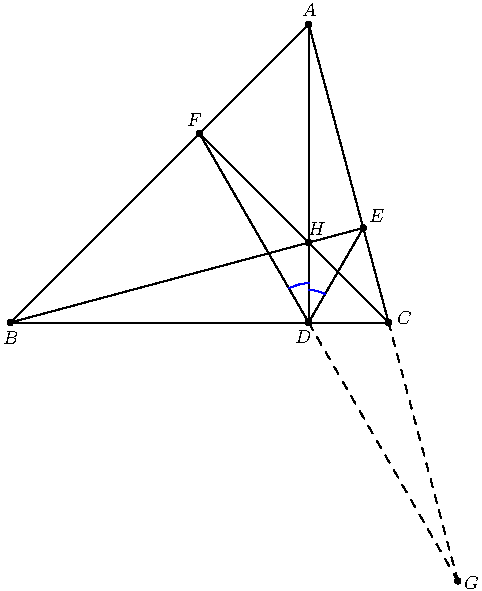
\includegraphics[scale=0.5]{p8-fig1.pdf}
\end{center}

\begin{soln}
设 $DF$ 交 $AC$ 于 $G$, 则由完全四边形的性质知 $(C,A;E,G)$ 构成调和点列.
The result then follows by the well-known property of 调和点列.

\begin{lem}[调和点列的性质]
设 $A,B,P,Q$ 是直线 $\ell$ 上的 $4$ 个点,
$X$ 是不在 $\ell$ 上的任意一点,
则以下 $4$ 个陈述, 任意 $2$ 个可以推出另外 $2$ 个:
\begin{enumerate}[label=\normalfont(\roman*)]
\ii $(A,B;P,Q)$ 构成调和点列.
\ii $XP$ 是 $\angle AXB$ 的内角平分线.
\ii $XQ$ 是 $\angle AXB$ 的外角平分线.
\ii $XP \perp XQ$.
\end{enumerate}
\end{lem}

\begin{center}
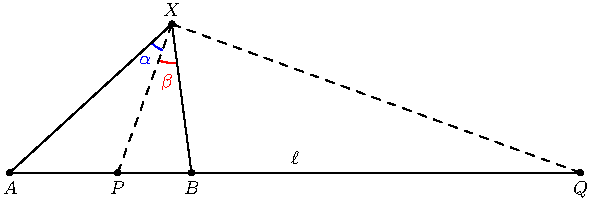
\includegraphics[scale=0.7]{p8-fig2.pdf}
\end{center}

\begin{proof}
这里只证明 (iv) 和 (i) 可以推出 (ii) 和 (iii).
设 $\alpha = \angle AXP, \beta=\angle BXP$, 由 (iv) 知
\begin{equation}
\label{eq11}
\frac{PA}{PB} = \frac{XA\sin\alpha}{XB\sin\beta}, \quad
\frac{QA}{QB} = \frac{XA\sin(90^\circ + \alpha)}{XB\sin(90^\circ - \beta)}.
\end{equation}
再由 (i) 知 $\frac{PA}{PB} = \frac{QA}{QB}$, 所以
\[\sin\alpha\cos\beta=\cos\alpha\sin\beta \iff \sin(\alpha-\beta) = 0.\]
因为 $X$ 不在直线 $\ell$ 上, 所以 $\alpha - \beta < 180^\circ$,
所以只能是 $\alpha = \beta$.
(ii) 和 (iv) 推出 (iii) 是显然的.
\end{proof}
\end{soln}

\begin{prob}
确定实系数多项式 $P(x)$ 使得多项式
$(x+1)P(x-1) - (x-1)P(x)$ 只有常数项.
\end{prob}

\begin{soln}
显然 $P(x)$ 为常数满足题意, 下面假设 $\deg P(x) \ge 1$.
设 $P(x) = \sum_{i=1}^n a_ix^i, \allowbreak Q(x) \defeq (x+1)P(x-1)-(x-1)P(x)
=P(x-1)+P(x) - x(P(x)-P(x-1))$.
显然 $P(x-1) + P(x)$ 的首项系数为 $2a_n$,
而 $x(P(x) - P(x-1))$ 的首项系数为 $na_n$,
所以只能是 $n=2$. 设 $P(x) = ax^2 + bx + c$,
则 $Q(x) = (b-a)x + (2c+a-b)$, 由此推出 $b=a$.
综上, 满足题意的实系数多项式为
\begin{equation}
\label{eq12}
P(x) = ax^2 + ax + c, \quad a,c \in \RR.
\end{equation}
\end{soln}

\begin{prob}
已知在 $\triangle ABC, \angle A < \angle B < 90^\circ$.
圆 $\Gamma$ 过点 $A,B,C$. 圆 $\Gamma$ 过点 $A,C$ 的两条切线交于 $P$.
直线 $AB$ 与 $PC$ 交于 $Q$.
若三角形 $ACP, ABC, BQC$ 有相同的面积,
求证 $\angle BCA = 90^\circ$.
\end{prob}

\begin{center}
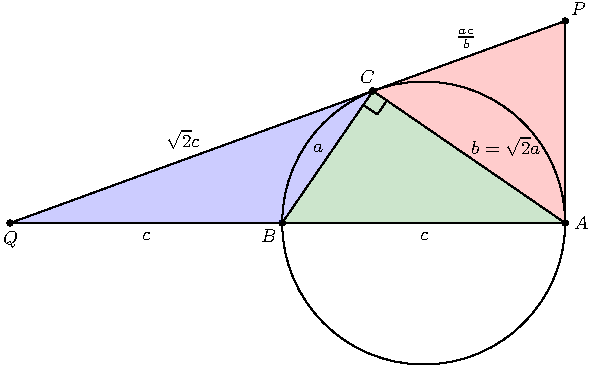
\includegraphics[scale=0.5]{p10.pdf}
\end{center}

\begin{soln}
我们用 $[XYZ]$ 表示 $\triangle XYZ$ 的面积. 我们有
\begin{equation}
\label{eq13}
\begin{aligned}
\angle PCA&=\angle PAC=\angle B,\\
\angle CPA&=180^\circ - 2\angle B,\\
\angle CQB&=180^\circ - \angle CPA-\angle BAP = \angle B - \angle A,\\
\angle QCB&=\angle A.
\end{aligned}
\end{equation}
因为 $[ACP] = [ABC]$, 且它们的高相等,
所以 $QB = c$. 因为 $QC$ 是切线,
所以 $QC^2 = QB\cdot QA \implies QC =\sqrt{2}c$.
由 $\triangle QCB \sim \triangle QAC$ 我们还可得出 $b = \sqrt{2}a$.
注意到
\[\frac{1}{2}BA\cdot BC\cdot \sin\angle B = [ABC]= [APC] = \frac{1}{2}AC\cdot AP\cdot \sin \angle B \implies PA=PC=\frac{ac}{b} = \frac{c}{\sqrt{2}}.\]
另一方面, 我们还有
\[\cos\angle B = \frac{\frac{1}{2}AC}{CP} = \frac{b}{\sqrt{2}c} = \frac{a}{c}.\]
这就证明了 $\angle BCA=90^\circ$.
\end{soln}

\section*{License}

\begin{itemize}
\ii 本作品采用\href{https://creativecommons.org/licenses/by-nc-sa/4.0/deed.zh}{署名-非商业性使用-相同方式共享 4.0 国际协议}.
\ii 笔者是自由创作人, 与澳门校际数学比赛官方无任何关联.
\ii One can download a copy of \href{https://www.dsedj.gov.mo/~webdsej/www/dsejnews/ce/result/tech/2021/math2021_sen_qust.pdf}{original test paper} from \href{https://portal.dsedj.gov.mo/webdsejspace/internet/Inter_main_page.jsp}{澳门教育及青年发展局官网}.
\ii 如果你发现这份参考答案中有任何错误, 请通过邮件告诉我.
\ii 为了修改各种小错误, 调整样式, 本作品可能还会经过多次修改,
建议从我的主页 \url{https://complex2math.com/problems} 处访问最新订正版.
\end{itemize}
\end{document}
